\chapter[Analysis of Geopoltical Regions]{Analysis of Geopolitical \\ Regions}
\label{app:maps}

This appendix outlines how network analysis can be performed on maps of geopolitical regions. 
The maps used as examples in this thesis are the communes of Switzerland (CH), the parishes and Westminster constituencies of Great Britain (GB) and the socio\--economic regions of the EU and EFTA (including both current and candidate countries at the time of writing), termed NUTS \cite{osmap,chmap,eumap}.
These are displayed in figures \ref{fig:ne7} and \ref{appfig:maps}.
%The shapefiles which give the maps of these geopolitical regions are available open source from the relevant institutions \cite{osmap,chmap,eumap}.

Geopolitical tilings can be thought of as consisting of tessellating administrative regions, where each administrative region on the map is defined by a boundary.
Regions can be said to be neighbours if they share at least one point anywhere along the boundary.
Vertices then form where three regions share a boundary and edges where two regions share a boundary.
In analogue to materials, the size of an administrative region is then defined as the number of neighbours (equivalent to the number of vertices or edges), as can be seen in figure \ref{appfig:mapdefb}.

\begin{figure}[tb]
	\centering
     
          \begin{subfigure}[b]{0.48\textwidth}
         \centering
         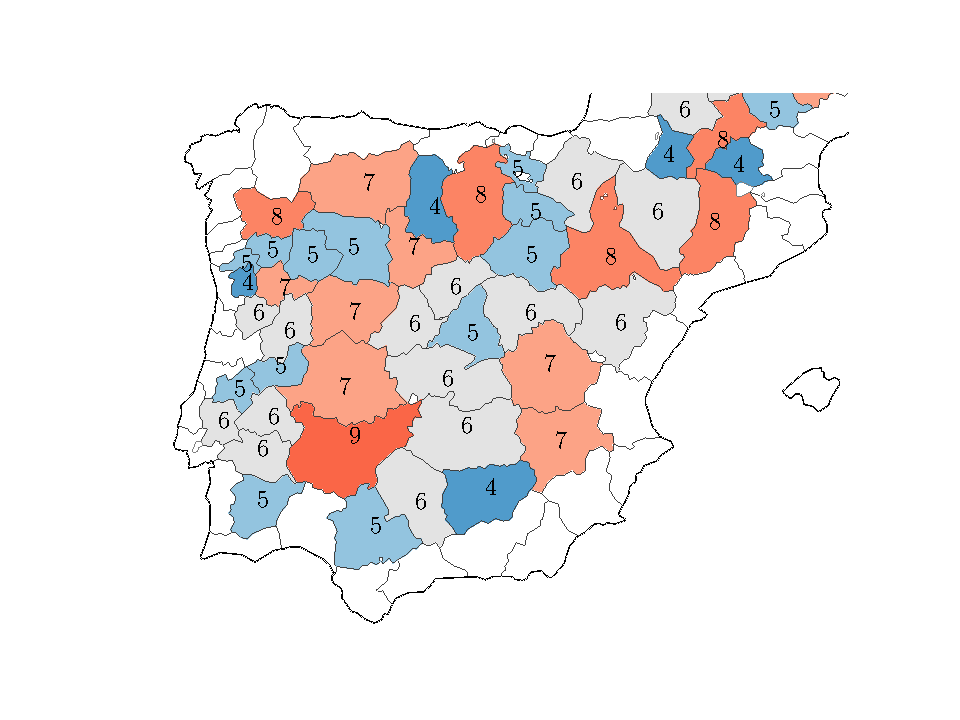
\includegraphics[width=0.8\textwidth]{./appendices/figures/region_count.pdf}
         \caption{}
         \label{appfig:mapdefb}
     \end{subfigure}
     \hfill
      \begin{subfigure}[b]{0.48\textwidth}
         \centering
         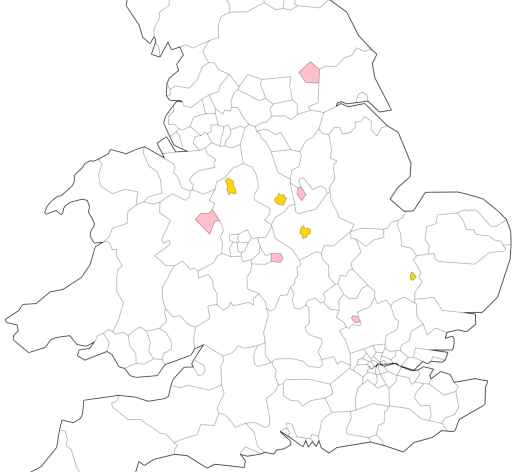
\includegraphics[width=0.8\textwidth]{./appendices/figures/map_defects.pdf}
         \caption{}
         \label{appfig:mapdefa}
     \end{subfigure}
     \hfill

	\caption{Panel (a) demonstrates how the number of neighbours of an administrative region defines the region size (as indicated by central numbers), in analogue with generic polygons. Panel (b) gives examples of the two defect types found in maps. Point defects (yellow) occur when a region is fully inscribed within another, and line defects (pink) when a region sits on the boundary between two others.}
	\label{appfig:mapdefects}
\end{figure}

Analysis of these geopolitical networks is slightly complicated by the possible presence of defects.
Defects arise when regions have $k<3$ neighbours, either as a result of small imperfections in the boundary data or from legitimate region arrangements.
For instance, if $k=0$, the region is an island, if $k=1$ a region is fully inscribed within another (usually indicative of a large urban area) and if $k=2$ a region sits on a ring edge.
Examples of these defects are given in figure \ref{appfig:mapdefa}.
As these maps are primarily for illustrative purposes, these defects can be simply discounted for the purposed of the network analysis.
A summary of the results from these geopolitical tilings is given in table \ref{tab:mapnet}.

\begin{table}[bt]
\caption{A network analysis of geopolitical results. The number of total and interior regions (without defects) are given for each map. The interior regions were then used to calculate the network properties.}
\label{tab:mapnet}
\centering
\begin{tabular}{ccccccccc}
\toprule
        Region & Total & Interior & $\ki$ & $p_6$ & $\mu_2$ & $r$ \\
        \midrule
        CH communes & 2379  & 2051 & 5.914    &    0.206     &   3.825   &    -0.151     \\
        GB parishes & 11663  & 10778  & 6.005    &    0.241    &    3.028   &    -0.163   \\
        GB West. const. & 654  & 455  &  5.930 &  0.251 & 3.019  & -0.110 \\
        EU/EFTA NUTS 2 & 387  & 145 & 5.897   &     0.283    &    1.913   &    -0.215   \\
        EU/EFTA NUTS 3 & 1617  & 972  & 5.910     &   0.271    &    2.531   &    -0.161   \\
        \bottomrule
\end{tabular}
\end{table}

\begin{figure}[tbp]
	\centering
     
      \begin{subfigure}[b]{0.48\textwidth}
         \centering
         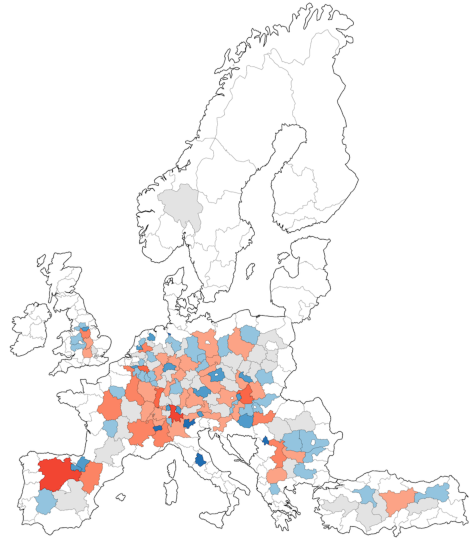
\includegraphics[width=1\textwidth]{./appendices/figures/eu2_lowres.pdf}
         \caption{EU/EFTA NUTS 2}
         \label{appfig:mapa}
     \end{subfigure}
     \hfill
      \begin{subfigure}[b]{0.48\textwidth}
         \centering
         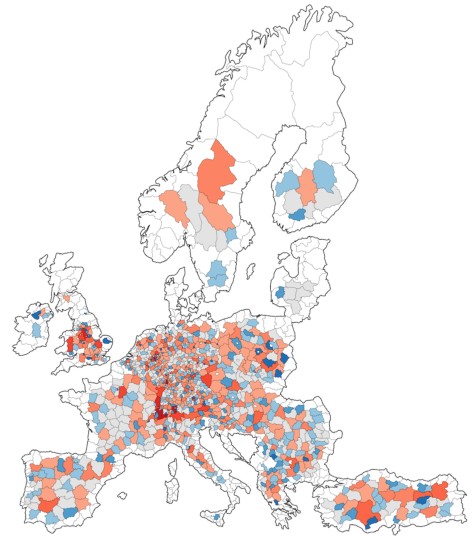
\includegraphics[width=1\textwidth]{./appendices/figures/eu3_lowres.pdf}
         \caption{EU/EFTA NUTS 3}
         \label{appfig:mapb}
     \end{subfigure}
	\vspace{0.5cm}     
     
      \begin{subfigure}[b]{0.48\textwidth}
         \centering
         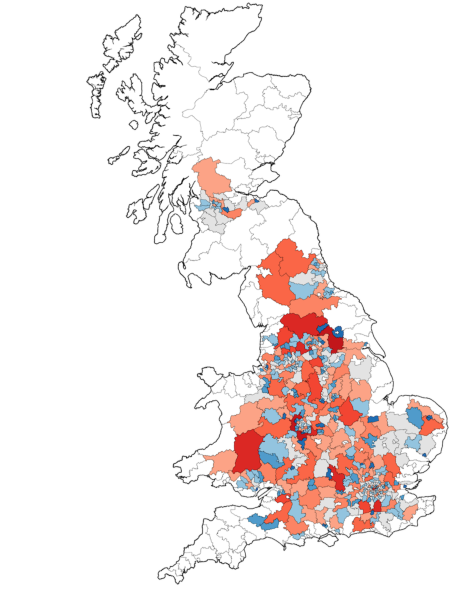
\includegraphics[width=0.9\textwidth]{./appendices/figures/gbw_lowres.pdf}
         \caption{GB Westminster constituencies}
         \label{appfig:mapc}
     \end{subfigure}
  	\hfill
      \begin{subfigure}[b]{0.48\textwidth}
         \centering
         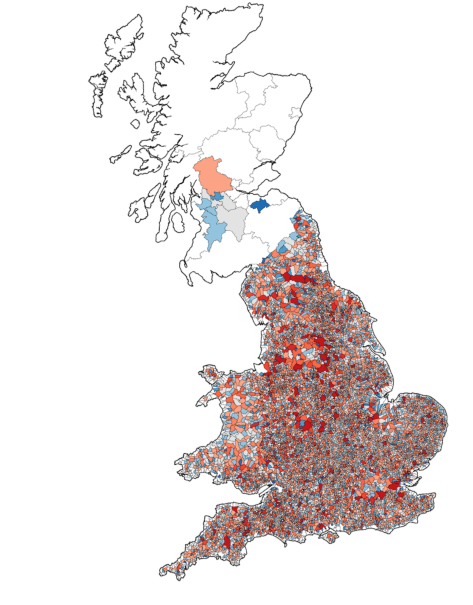
\includegraphics[width=0.9\textwidth]{./appendices/figures/gbp_lowres.pdf}
         \caption{GB parishes}
         \label{appfig:mapd}
     \end{subfigure}

	\caption{Geopolitical regions used for network analysis (as indicated in captions), in addition to the communes of Switzerland in figure \ref{fig:ne7}. Regions on sea frontiers are neglected, as are those completely surrounded by another region (shaded white).}
	\label{appfig:maps}
\end{figure}